\head{Ноябрь}{Листок 4. Теория чисел. Уровень 1.}

\begin{thm}
    Докажите, что, если $a \del b$, а $b \del c$, то $a \del c$.
\end{thm}

\begin{thm}
    Пусть $a \del c$, а $b \del d$. Докажите, что $(ab) \skdel (cd)$.
\end{thm}

\begin{thm}
    Даны два числа $a$ и $b$ такие, что $a \del b$. Можно ли утверждать, что $a^n \del b^n$ при любом натуральном $n$?
\end{thm}
    
\begin{thm}
    Известно, что $(ab) \skdel c$ и что $(a+b) \skdel c$. Докажите следующее\footnote{Подсказка: воспользуйтесь формулами сокращённого умножения.}:
    \par 
    а)~$(a^2+b^2) \skdel c$ 
    \par 
    б)~$(a^3+b^3) \skdel c^2$
\end{thm}
    
\begin{thm}
    Докажите, что, если $a^2  \skdel (a + b)$, то и $b^2  \skdel (a + b)$.
\end{thm}

\begin{thm}$^n$ \label{4.1 thm1}
    Докажите, что если $a_1 \del c$, $a_2 \del c$, …, $a_{n-1} \del с$, но $a_n \ndel c$, то $(a_1 + a_2 + ... + a_n)~\ndel c$.
\end{thm}

\begin{thm}
    Глеб на каждой следующей перемене съедает в два раза больше бутербродов с сыром, чем на
предыдущей. Может ли он за две перемены подряд съесть а) 2010 бутербродов? б) 2012?
\end{thm}

\begin{thm}
    В Радужном городе живут 13 чебурашек. У каждого чебурашки есть 3 воздушных шарика:
1 красный, 1 синий и 1 зелёный. Могут ли чебурашки поменяться своими шариками друг с другом так,
чтобы у каждого оказались шарики только какого-либо одного цвета?
\end{thm}

\begin{thm}$^n$ \label{4.1 thm2}
    Группа детского сада построилась парами. Известно, что в каждой паре у одного в три раза больше конфет, чем у второго. Может ли общее число конфет быть равным 2007?
\end{thm}

\begin{thm}
    В одном из подъездов 8-этажного дома на 1 этаже находятся квартиры от № 97 до № 102.
На каком этаже и в каком (по номеру) подъезде находится квартира 178? (на всех этажах одинаковое
число квартир и все подъезды устроены одинаково)
\end{thm}

\setlength{\intextsep}{0pt}
\begin{figure}[h]
\begin{minipage}[h]{0.84\linewidth}\setlength{\parindent}{1.5em}
\begin{thm}
Знайка собирал свои книги в путешествие. Он упаковал все книги в
пачки по 4 штуки. Потом он заметил, что все книги можно упаковать по 6 книг в
каждую пачку. Наблюдавший за всем этим Незнайка воскликнул: «Слушайте, так
ведь если можно упаковать все книги по 4 и по 6 книг в пачку, значит можно
уложить также все книги по 24 в каждой пачке!». Прав ли Незнайка?
\end{thm}

\begin{thm}
    Астроном Стекляшкин тоже задумал упаковать свои книги и отнести на
чердак. Он обнаружил, что если их связывать по 4, по 5 или по 6 книг в пачку, то
каждый раз остается одна лишняя книга, а если по 7 книг в пачку, то лишних книг
не остается. Сколько, самое меньшее, книг хотел отнести на чердак Стекляшкин?
\end{thm}

\end{minipage}
\begin{minipage}[h]{0.15\linewidth}
    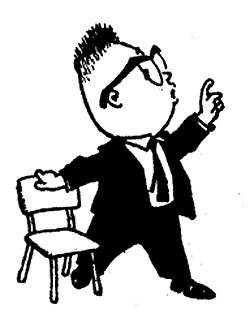
\includegraphics[width=0.9\columnwidth]{./img/znaika}
\end{minipage}
\end{figure}
\setlength{\intextsep}{12pt}

\begin{thm}
    Прочитав листок «Делимость» и не решив ни одной задачи, Гоша рассердился разорвал его
    на 7 частей. Подумав, он взял некоторые куски и порвал каждый еще на 7 частей, и так далее…. В какой-
    то момент ему это надоело и он ушел в буфет. В это время в класс заглянула Юля и обнаружила 2009
    кусков. Она утверждает, что часть кусков Гоша успел потерять. Можно ли ей верить?
\end{thm}

\begin{thm}
    Лиза решила склеить порванный листок. Она нашла все недостающие кусочки и стала
склеивать всё обратно. Сначала она склеила вместе 4 куска, потом ещё 4 куска, и так
далее… Но, не склеив до конца весь листок, она обнаружила, что ей пора в музыкальную школу. Поэтому она оставила все куски и ушла. Могло ли в результате всех стараний Лизы остаться ровно 2009 кусков?
\end{thm}

\begin{thm}
    Андрей приобрёл в магазине несколько бутылочек лимонада «Black Death» по 35 руб. 77 коп.,
несколько шоколадок по 14 руб. и несколько конфет по 6 руб. 30 коп. за штуку. На кассе ему сообщили, что он должен заплатить 1000 руб. Докажите, что подсчёт произведен неверно.
\end{thm}

\begin{thm}
    Найдите последнюю цифру числа: а) $1999^{1999}$; б) $333^{333}$; в) $2007^{2007}$.
\end{thm}

\begin{thm}$^n$ \label{4.1 thm3}
    Петя купил общую тетрадь объёмом 96 листов и пронумеровал все её страницы по порядку числами от 1 до 192. Вася вырвал из этой тетради 25 листов и сложил все 50 чисел, которые на них написаны. Могло ли у него получиться 2006?
\end{thm}

\textbf{\textit{Внимание! В этот раз в этой части три письменных задачи - \ref{4.1 thm1}, \ref{4.1 thm2} и \ref{4.1 thm3}.}}